%!TEX root = ../main.tex
\chapter{Introduzione}\label{chp:introduction}

Ad oggi l'avanzamento della genomica — branca della biologia molecolare che si occupa di studiare il genoma degli esseri viventi — si è rivelato notevolmente significativo al fine di approfondire e comprendere malattie legate alle mutazioni del genoma degli individui. Si stima che solamente una percentuale tra l'1\% e il 2\% del DNA contiene i \textsl{geni}, ovvero particolari regioni che contengono tutte le informazioni necessarie per la sintesi degli aminoacidi che poi comporranno le proteine\,\cite{sahu2011identification, pollard2022cell}. Ciò nonostante, la quasi totalità dei disturbi genomici è dovuta alle mutazioni nelle regioni non codificanti\,\cite{zhang2015non} — dette \textsl{varianti non codificianti}. Le mutazioni in queste zone del genoma, che apparentemente svolgono funzioni marginali, sono responsabili dello sviluppo di disturbi importanti, come le \textsl{malattie mendeliane}\footnote{Le malattie mendeliane, causate dalla mutazione di un singolo gene, includono la fibrosi cistica e il morbo di Huntington.}\,\cite{french2020role, chial2008mendelian}, l'epilessia\,\cite{pagni2022non}, malattie cardiovascolari\,\cite{kapoor2014enhancer, zhang2015non} e soprattuto tumori — tra cui il cancro del colon-retto e tumore al seno\,\cite{khurana2016role, tian2019systematic, bojesen2013multiple, michailidou2017association}.

Risulta quindi vitale continuare a studiare gli effetti che le varianti non codificanti in sequenze genomiche hanno sugli individui. Proprio a questo proposito, con l'avvento dell'intelligenza artificiale, in particolare del \textsl{deep learning}, si continuano a trovare e perfezionare soluzioni che permettano di delineare sempre con più precisione il ruolo che hanno le mutazioni nelle regioni non codificanti del DNA.\@ Grazie a queste nuove tecnologie, la \textsl{genomica funzionale} — area della genomica che si interessa a descrivere le relazioni che ci sono tra i componenti di un sistema biologico, come geni e proteine\,\cite{caudai2021ai} — ha avuto un forte impulso nell'approfondire le varianti non codificanti ma rimangono ancora significative lacune nella comprensione riguardante la relazione tra mutazioni genetiche ed espressione genica. L'utilizzo di tecniche di deep learning quindi cruciale per continuare la ricerca; a questo proposito, nel presente elaborato accademico verranno descritti e paragonati tre \textsl{tool} che utilizzano le \textsl{reti neurali convoluzionali} per predire l'effetto delle varianti non codificanti su sequenze genomiche: DeepSEA\,\cite{zhou2015predicting}, Basset\,\cite{kelley2016basset} e DeepSATA\,\cite{ma2023deepsata}.



\section{Background}

La cellula è l'unità fondamentale della vita. La cellula è una piccola miscela acquosa con componenti chimici, racchiusi in una mambrana, e possiede l'eccezionale capacità di replicarsi. Il primo elemento che permette di distinguere le cellule è la presenza di un nucleo. Vengono definite \textsl{procarioti} le cellule senza nucleo — che sono le più diffuse e compongono organismi unicellulari come i batteri e gli archei — mentre sono chiamate \textsl{eucarioti} le cellule che contengono un nucleo — le quali sono in genere più grandi e più complesse e costituiscono forme di vita multicellulari come animali piante e funghi\,\cite{alberts2015essential}.

All'interno della cellula eucariote (illustrazione\,\ref{fig:cell}), immersi nel \textsl{citoplasma}, sono presenti diversi \textsl{organuli}, i quali svolgono una particolare funzione ciascuno. I \textsl{mitocondri} sono gli organuli più diffusi all'interno del \textsl{citoplasma}. Il loro compito è quello di generare energia chimica per la cellula: attraverso il processo di ossidazione di zuccheri e grassi, viene creata una sostanza che viene utilizzata nella maggior parte delle attività cellulari\footnote{Questa sostanza è detta \textsl{adenosintrifosfato} o ATP ed ha una struttora simile ad un nucleotide: è infatti composta dall'Adenina, da uno zucchero e da tre gruppi fosfati.}; questo processo è anche chiamato \textsl{respirazione cellulare} perchè consumando l'ossigeno viene rilasciata anidride carbonica\,\cite{alberts2015essential, chinnery2003mitochondria}. Oltre ad essere la fonte energetica primaria della cellula, i mitocondri hanno anche importanti ruoli nella regolazione del metabolismo, del ciclo cellulare, delle risposte antivirali e anche della morte della cellula\,\cite{mcbride2006mitochondria}.

Il \textsl{reticolo endoplasmatico} è invece un organulo molto esteso e svolge molteplici funzioni. Tra queste compiti rientrano quelli di traslocazione di proteine e il ripiegamento delle proteine (\textsl{protein folding})\,\cite{alberts2015essential, voeltz2002structural}. I \textsl{lisosomi} si occupano di degradare e riciclare gli scarti cellulari e giocano un ruolo fondamentale per l'omeostasi della cellula\footnote{Con omeostasi cellulare si intende l'insieme di meccanismi necessari per mantenere ad un livello ottimale le funzioni della cellula.}, il suo sviluppo e il suo invecchiamento\,\cite{ballabio2016awesome, yang2021lysosome, dell2000lysosome}. Infine, i \textsl{perossiomi} sono delle piccole vescicole che forniscono un ambiente protetto per gestire molecole tossiche come gli acidi grassi i quali sono smaltiti tramite la $\beta$-ossidazione\,\cite{alberts2015essential, islinger2012peroxisome, islinger2018peroxisome}.

\begin{figure}[h]
    \centering
    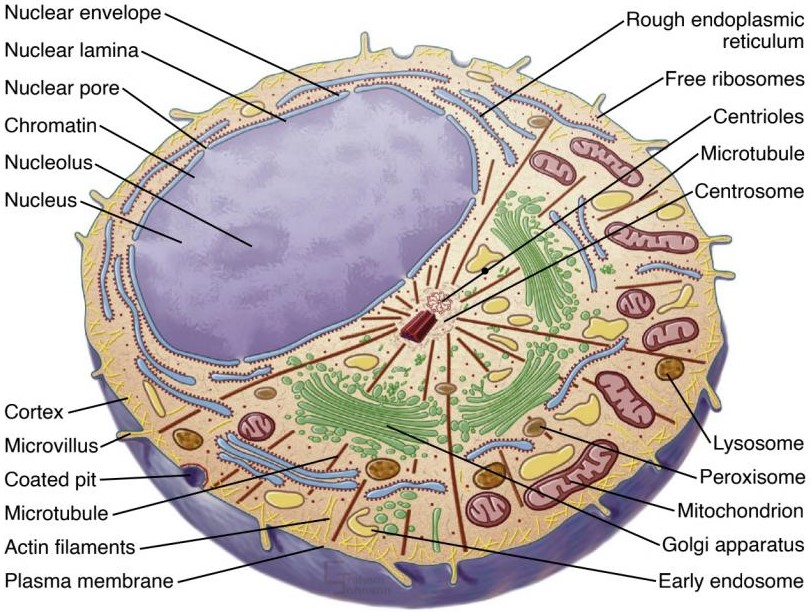
\includegraphics[width=.65\textwidth]{assets/cell.jpg}
    \caption[Rappresentazione schematica della cellula eucariote.]{Rappresentazione schematica della cellula eucariote; si possono notare i principali organuli tra cui i mitocondri, lisosomi e perossiomi, il reticolo endoplasmatico, e il nucleo\,\cite{pollard2022cell}.}\label{fig:cell}
\end{figure}

L'organulo più importante della cellula rimane il \textsl{nucleo}. Racchiuso nell'\textsl{involucro nucleare}, all'interno di questo organulo sono presenti tutte le informazioni genetiche, racchiuse in una lunga molecola di acido desossiribonucleico (comunemente noto come DNA), che, una volta impacchettato forma il \textsl{cromosoma}\,\cite{pollard2022cell, alberts2015essential}. La molecola di DNA è una struttura a doppia elica formata da \textsl{nucleotidi}. Osservando l'illustrazione\,\ref{fig:dna}, i nucleotidi sono composti a loro volta da tre elementi fondamentali: una \textsl{base azotata}, uno \textsl{zucchero} e un \textsl{gruppo fosfato}\footnote{I gruppi fosfati hanno una carica negativa e forniscono alla molecola le proprietà di un acido.}. Le basi azotate sono quattro — Adenina (A), Citosina (C), Guanina (G) e Timina (T) — e si uniscono tra loro mediante dei legami ad idrogeno e secondo un preciso criterio: l'Adenina si lega solamente con la Timina (formando il legame \textit{AT}) mentre la Citosina si unisce solo con la Guanina (creando la coppia \textit{CG})\,\cite{fonseca2000hydrogen, sahu2011identification}. 

\begin{figure}[h]
    \centering
    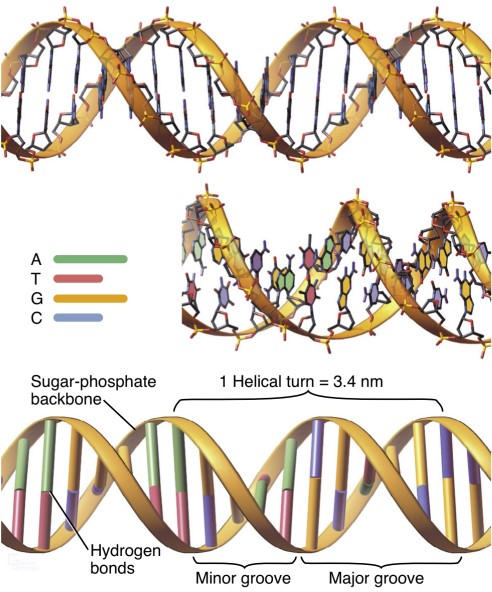
\includegraphics[width=.5\textwidth]{assets/dna.jpg}
    \caption[Rappresentazione schematica del DNA.]{Rappresentazione schematica del DNA;\@ si possono osservare le coppie di basi azotate, legate tra loro attraverso gli zuccheri e i gruppi fosfati\,\cite{pollard2022cell}.}\label{fig:dna}
\end{figure}

\noindent 




\begin{figure}[h]
    \centering
    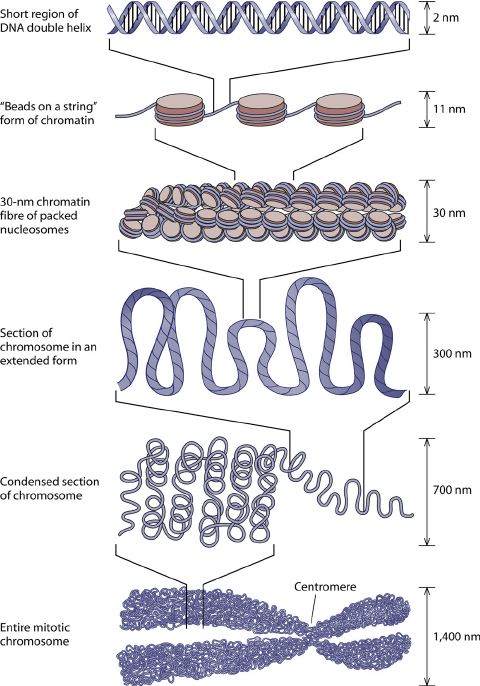
\includegraphics[width=0.6\textwidth]{assets/dna-packaging.png}
    \caption[Il processo di impacchettamento del DNA.]{Il processo di impacchettamento del DNA\,\cite{jansen2011nucleosome}.}\label{fig:dna-packaging}
\end{figure}



\todo{I \textsl{ribosomi} si occupano di accelerare la sintesi delle proteine usando le sequenze di nucleotidi del \textsl{RNA messaggero} (mRNA) per specificare la sequenza di aminoacidi }
\todo{Parla dei nucleoli\,\cite{pederson1998plurifunctional}}
\todo{parla dei geni, delle parti del gene in modo da spiegare bene le varianti non codificanti. Se vuoi parla anche della funzione del dna del creare proteine descrivendo in breve il DNA}
\todo{parla anche di come il DNA è salavto dei cromosmi in agglomarati}
\todo{DNA replication\,\cite{bell2002dna}}

\section{Cenni storici}
\todo{
    C'è sto bell'articolo che racconta per bene la situa\cite{crick1954complementary, watson1953molecular, li2021cell}. Qua ci puoi buttare dentro anche la questione meme del junk DNA così pushi per bene le citazioni goliardiche. Cita il libro\,\cite{pollard2022cell} che descivre a cosa serve il dna (pagina 10)
}
\todo{ Sto libro parla anche della scopetrta delle cellule\cite{alberts2015essential}}


\section{Stato dell'arte}

\todo{parla dei tool e quanti ne sono uscit per letsgoscare le cose. Parla delle diversi vantaggi che AI ha portato nel letsgosky. Butta dentro deepvirfinder a anche alphafold perche fa figo\cite{ren2020identifying}}
\todo{anche esmpi di DNA folding}


% https://books.google.it/books?hl=it&lr=&id=Cg4WAgAAQBAJ&oi=fnd&pg=PP1&dq=Introduction+to+cell+biology&ots=yg4LdM46O3&sig=FkW8Ei_rOFccb96Sw3A28QsHuFo&redir_esc=y#v=onepage&q=Introduction%20to%20cell%20biology&f=false

% https://books.google.it/books?hl=it&lr=&id=mXiiEAAAQBAJ&oi=fnd&pg=PP1&dq=cellular+biology&ots=8O1TrOZBXp&sig=fqZhVnT0H-I3qEu1iPk4v2nvZi8&redir_esc=y#v=onepage&q=cellular%20biology&f=false

% https://books.google.it/books?hl=it&lr=&id=z4BDRcLrekMC&oi=fnd&pg=PR19&dq=cell+nucleus+organization&ots=wiXN8JbVpC&sig=oviVqMKJqsvcYwe4X37tQM28P3Y&redir_esc=y#v=onepage&q=cell%20nucleus%20organization&f=false
